\documentclass[tikz]{standalone}

\usepackage{tikz}

\usetikzlibrary{arrows, automata, topaths, calc, shapes.geometric}

\begin{document}

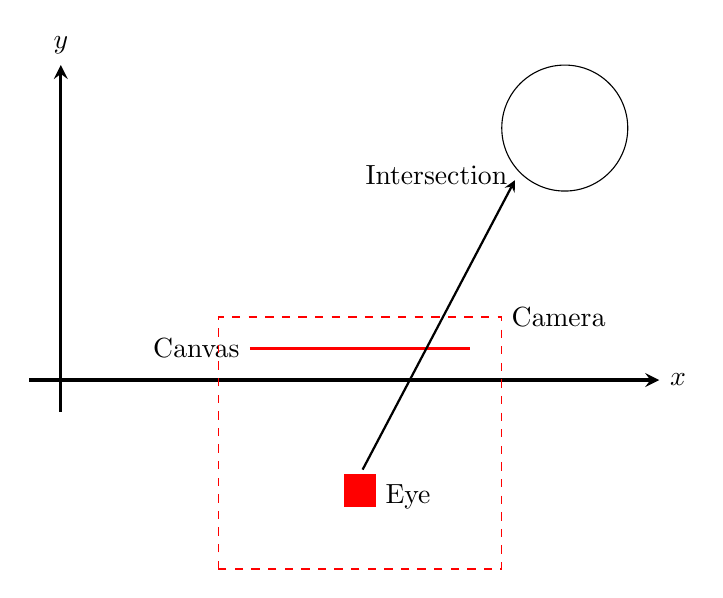
\begin{tikzpicture}[
        scale=0.4,
        axis/.style={very thick, ->, >=stealth},
        important line/.style={thick},
        dashed line/.style={dashed, thin},
        pile/.style={thick, ->, >=stealth, shorten <=2pt, shorten >=2pt},
        every node/.style={color=black}]

    % axis
    \draw[axis] (-1,0)  -- (19,0) node(xline)[right] {$x$};
    \draw[axis] (0,-1) -- (0,10) node(yline)[above] {$y$};

    \draw (16,8) circle (2);

    \filldraw[red] (9,-4) rectangle (10,-3) node(eye)[below right]{Eye};
    \draw[red, thick] (6,1) node(canvas)[left] {Canvas} -- (13,1);
    \draw[red, dashed] (5,-6) rectangle (14,2) node(camera)[right]{Camera};
    \draw [pile] (9.5,-3) -- (14.5,6.5) node(hit)[left]{Intersection}; 
\end{tikzpicture}
\end{document}
